\documentclass[11pt]{article}
\usepackage{fullpage}
\usepackage{amsmath}
\usepackage{mathtools}
\usepackage{esint}
\usepackage{cancel}
\usepackage{graphicx}
\usepackage{float}
\linespread{1.1}
\allowdisplaybreaks
\usepackage{color}
\usepackage{listings}
\usepackage{subfigure}
\usepackage{multicol}
\usepackage{xcolor}
\usepackage{sectsty}
\definecolor{darkblue}{RGB}{10,0,100}
\definecolor{otherblue}{RGB}{0,70,200}
\sectionfont{\color{darkblue}} 
\subsectionfont{\color{otherblue}}  


\begin{document}

\title{ACT370  \\ Financial Principles for Actuarial Science II}
\author{Michael Boyadjian}
\maketitle
\pagebreak

\tableofcontents

\pagebreak

\bigskip
\bigskip
\bigskip


\section{Introduction to Pricing, Financial Instruments, and Derivatives}
\hrule \vspace{15pt}
\subsection{Derivatives}
There are several ways to define a derivative:
\begin{itemize}
\item \underline{\textbf{Textbook}}: An agreement between two parties which has a value determined by the price of something else
\item \underline{\textbf{US GAAP}}: A financial instrument or other contract with the following characteristics 
\begin{enumerate}
\item Has (1) one or more underlyings and (2) one or more notional amounts of payment provisions or both
\item Requires no initial net investment or an initial net investment that is smaller than would be required for other types of contracts that would be expected to have a similar response to changes in market factors
\item Terms require or permit net settlement, it can be readily settled net by a means outside the contract, or it provides for delivery of an asset that puts the recipient in a position not substantially different from net settlement
\end{enumerate}
\item \underline{\textbf{IFRS IAS39}}:  A financial instrument with the following characteristics 
\begin{enumerate}
\item Value changes in response to a change in price of, or index on,  a specified underlying financial or non-financial item or other variable
\item Requires no, or comparatively little initial investment
\item To be settled at a future date
\end{enumerate}
\end{itemize}
Derivatives can also be classified as several different types:
\begin{itemize}
\item \textbf{Freestanding}: Options, futures, forwards, swaps, swaptions, etc.
\item \textbf{Exchange Traded}: Options, futures
\item \textbf{Over-the-Counter}: Options, forwards
\item \textbf{Embedded}: Bond with a coupon defined by a ratio of FX rates
\end{itemize}


\subsection{Forward Contracts}
Forward contracts are an obligation to buy/sell an underlying asset in the future, at a price set today. This specifies the following:
\begin{itemize}
\item Features and quantity of the asset being delivered
\item Delivery logistics,  such as time, date, and place
\item Price the buyer will pay at the time of delivery
\end{itemize}
\pagebreak
The \textbf{Payoff} of a contract is its value at expiration. This could be either a long forward or short forward:
\begin{itemize}
\item \textbf{\textit{Long Forward}} $=$ $Spot$ $Price$ $at$ $Expiration$ $-$ $Forward$ $Price$
\item \textbf{\textit{Short Forward}} $=$ $Forward$ $Price$ $-$ $Spot$ $Price$ $at$ $Expiration$ 
\begin{center}
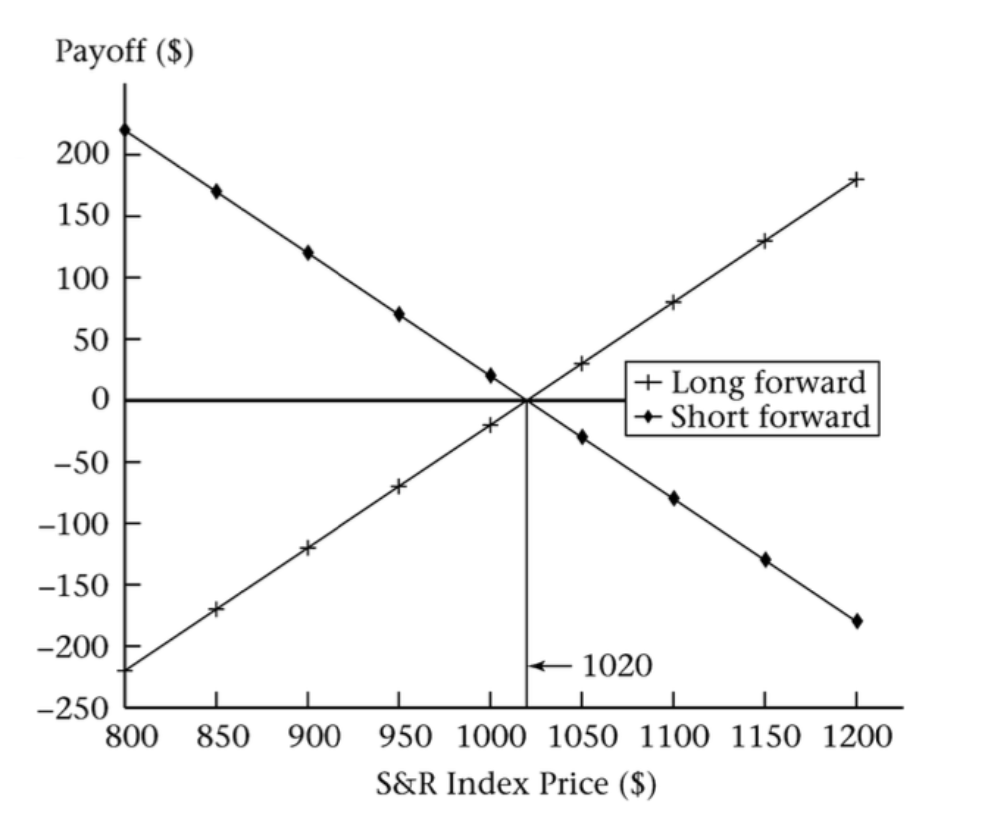
\includegraphics[scale=0.4]{images/forwards.png} 
\end{center}
\end{itemize}
Some additional considerations when looking at forward contracts include the following:



\subsection{Options}


\pagebreak
\section{Binomial Asset Pricing Model}
\section{Lognormal Stock Price Model}
\section{Black-Scholes Formula}
\section{Exotic Options}
\section{Interest Rate Derivatives}


\end{document}
